\documentclass[main.tex]{subfiles}
\begin{document}

%\custompart{Quantifier l'\hetero d'une tumeur à partir d'une image}{Comment ? Par quel biais? Exploration de différents critères.}{Dans cette partie, on propose d'examiner en détail le caractère \heterogene de nos images - les images médicales ainsi que les images produites numériquement avec le modèle EDP. Dans un premier temps, nous présenterons la construction d'histogrammes des niveaux de gris contenus dans l'image. Dans un second temps, nous décrirons ces histogrammes par un mélange de gaussienne. Enfin ce mélange gaussien sera utilisé pour calculer différents critères qui seront comparés. }

%\chapter{Construction des histogrammes de niveaux de gris}
%\chapter{Fit des histogrammes}
%\todo[noline]{On peut employer le mot "fit" ?}


\chapter{Critères quantifiant l'\hetero.}
%\lettrine[lines=2, lhang=0.33, loversize=0.25]{$\mathscr{D}$}{ans} 
\lettrine[lines=2, lhang=0.33, loversize=0.25]{D}{ans} 
tout ce chapitre, on considère l'approximation en un mélange de deux  gaussiennes d'un histogramme de niveau gris. Ce mélange gaussien est entièrement décrit par les paramètres suivants:
\begin{itemize}
\item $c_1, c_2$ : Centre des gaussiennes.
%% Sans pertes de généralité on peut admettre que l'on a ordonné les gaussienne \ie $c_1<c_2$.
\item $\sigma_1,\sigma_2$ : Ecart-type de chacune des gaussiennes
\item $w_1,w_2$ : Poids associées aux gaussiennes dans le mélange ($w_1+w_2=1$)
\end{itemize}
On peut ainsi définir plusieurs quantités caractéristiques :
\begin{itemize}
\item $h_1,h_2$ : Hauteur des gaussiennes. Elles sont données par $h_i = \frac{w_i}{\sigma_i\sqrt{2\pi}}$
\end{itemize}
Notons $\Delta$ l'opérateur de différence défini par :
\begin{equation}
\label{eq:operateur_delta_gaussienne}
\Delta :  u \longmapsto \Delta u := u_2 - u_1.
\end{equation}
Ainsi les quantités suivantes pourront s'avérée intéressantes à étudier : $\Delta c$, $\Delta \sigma$,  $\Delta \sigma^2$, $\Delta h$, $\Delta w$ représentant respectivement l'écart entre les centres, la différence d'écart-type, la différence des variances, la différence des hauteurs et la diffirences des poids. On pourra aussi regarder le ratio des quantités :
\begin{equation}
\label{eq:operateur_quotient_gaussienne}
Q :  u \longmapsto Qu := \dfrac{ \min( u_2 , u_1) }{ \max( u_2 , u_1)  }.
\end{equation}

\section{Définition d'une fonction objectif à reproduire}
Afin de correctement traduire l'\hetero, il est nécessaire de fournir une fonction objectif que notre critère devra reproduire au mieux. Ainsi, j'ai décidé de catégoriser l'ensemble des scanners de nos patients. Le partage des scanners est ainsi fait en 5 catégories, en associant à chaque catégorie une valeur de l'\hetero $\mathscr{H}$ :
\begin{itemize}
\item $\mathscr{H}=0.9$ : très \heterogene
\item $\mathscr{H}=0.7$ : plutôt \heterogene
\item $\mathscr{H}=0.5$ : cas intermédiaire ou difficile à caractériser
\item $\mathscr{H}=0.3$ : plutôt homogène
\item  $\mathscr{H}=0.1$ : très homogène
\end{itemize}
Après appréciation visuelle \footnote{\samepage Cette appréciation visuelle reste ma perception personnelle même si je me suis efforcer de rester le plus objectif possible. Mettre à contribution les membres de l'équipe de recherche par exemple, pour leur demander une catégorisation aurait pu permettre de confronter l'évolution de l'\hetero au cours du temps que je perçois à celle que perçoivent les autres. La fonction objectif finale pourrait ainsi être la moyenne de celles que chacun obtient. On aurait donc un peu plus de nuances : des valeurs intermédiaires aux 5 paliers notamment ainsi que des barres d'erreur pour chaque valeur}
%(la fonction objectif sera appelée \hetero visuelle)
, voici ce que donne les fonctions objectifs pour $\mathscr{H}$ (\cf  Figure~\ref{fig:hetero_visuelle} ).

\begin{figure}
\subfloat[\label{fig:hetero_objectif_Nber}\Nber]{\includegraphics[width=0.48\textwidth]{graph_hetero/dcm_Nber/00-note_hetero.png}}
\subfloat[\label{fig:hetero_objectif_Chen}\Chen]{\includegraphics[width=0.48\textwidth]{graph_hetero/dcm_Chen/00-note_hetero.png}}
\caption{\label{fig:hetero_visuelle}Fonction objectif de l'\hetero}
\end{figure}

Notons que \Nber est encore ici un cas très représentatif de ce que l'on cherche à étudier \ie corrélation entre \hetero et rechute imminente. En effet, ici l'\hetero croit avant même que le volume tumorale ne réaugmente, signe de la reprise d'activité cellulaire sur le pourtour de la métastase. Le coeur reste nécrosé et donc l'\hetero est accrue. Lorsque le volume tumorale fini par augmenter, le tissu proliférant à, en grande partie (si le centre de la tumeur est suffisament vascularisé), recoloniser la zone nécrosée. La croissance de la métastase est alors synonyme d'homogénéisation, puisque l'ensemble de la surface tumorale tend à être proliférante. Une homogénéisation a également lieu lorsque le traitement est efficace. Dans ce cas-ci, l'ensemble de la tumeur tend à être nécrosée.


Bien que nous ayons 2 patients à notre disposition, je m'efforcerais de construire un critère qui reproduira convenablement la fonction objectif pour \Nber uniquement. Le second patient, \Chen, sera gardé pour valider le ou les critère(s) retenu(s) et non pour le ou les construire. L'idéal serait bien sûr d'avoir à notre disposition une plus large cohorte de patient...

\section{Premiers essais de critères}
Examinons à présent, les informations que fournissent les quantités suivantes (qui pourraient être des quantificateurs de l'\hetero):
\begin{align}
\mathcal{H}_1 =& \frac{|\Delta c |}{256}, \\
\mathcal{H}'_1 =& 1-Qc, \\ %%1-\frac{ \min(c_1,c_2) }{\max(c_1,c_2)}, \\
\mathcal{H}'_2 =& \left| \frac{\Delta c / 256 }{\Delta h}\right|, \\
%% \mathsrc{A} & %%% on ne peut pas utiliser mathsrc ici ...
\mathcal{H}_3 =& Qw, \\ %%\frac{ \min (w_1,w_2) }{ \max (w_1,w_2) },  \\
\mathcal{H}'_3 =& |\Delta w|, \\
\mathcal{H}_8 =& |\Delta h|, \\
\mathcal{H}'_8 =& Qh. %%\frac{ \min (h_1,h_2) }{ \max (h_1,h_2) },
\end{align}

\begin{figure}[htpb]
\subfloat[\label{fig:critere_dc}Critères basés sur $\Delta c$]{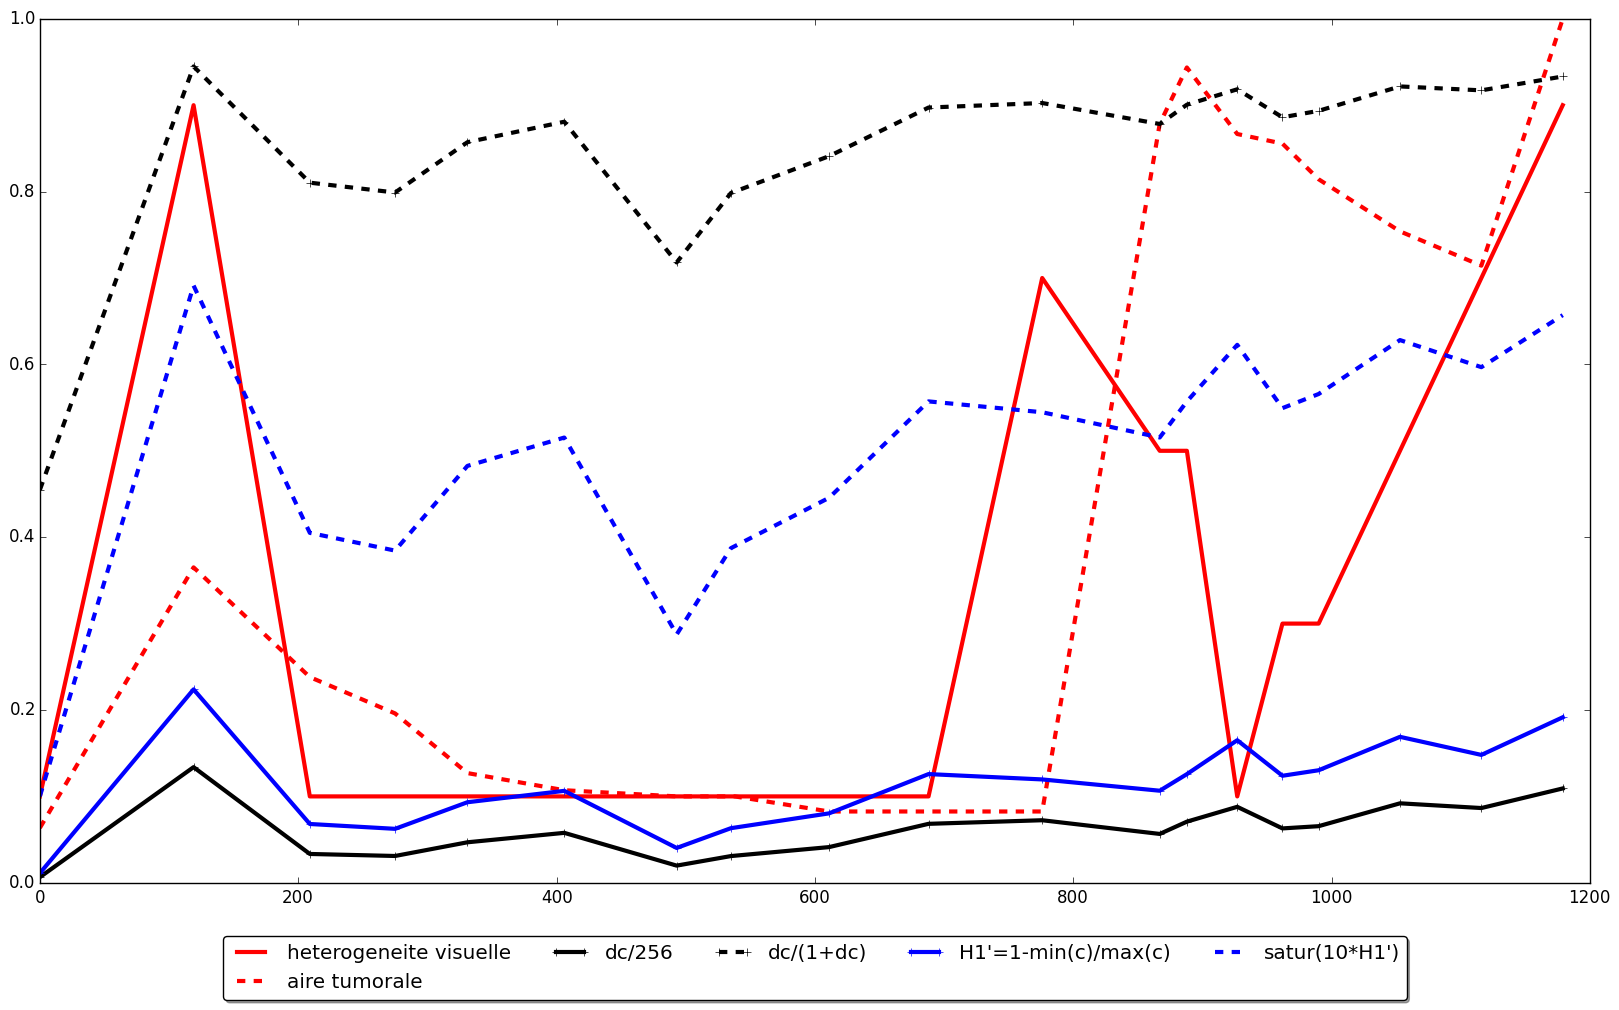
\includegraphics[width=0.48\textwidth]{graph_hetero/dcm_Nber/01-dc.png}}
\subfloat[\label{fig:critere_dh}Critères basés sur $\Delta h$]{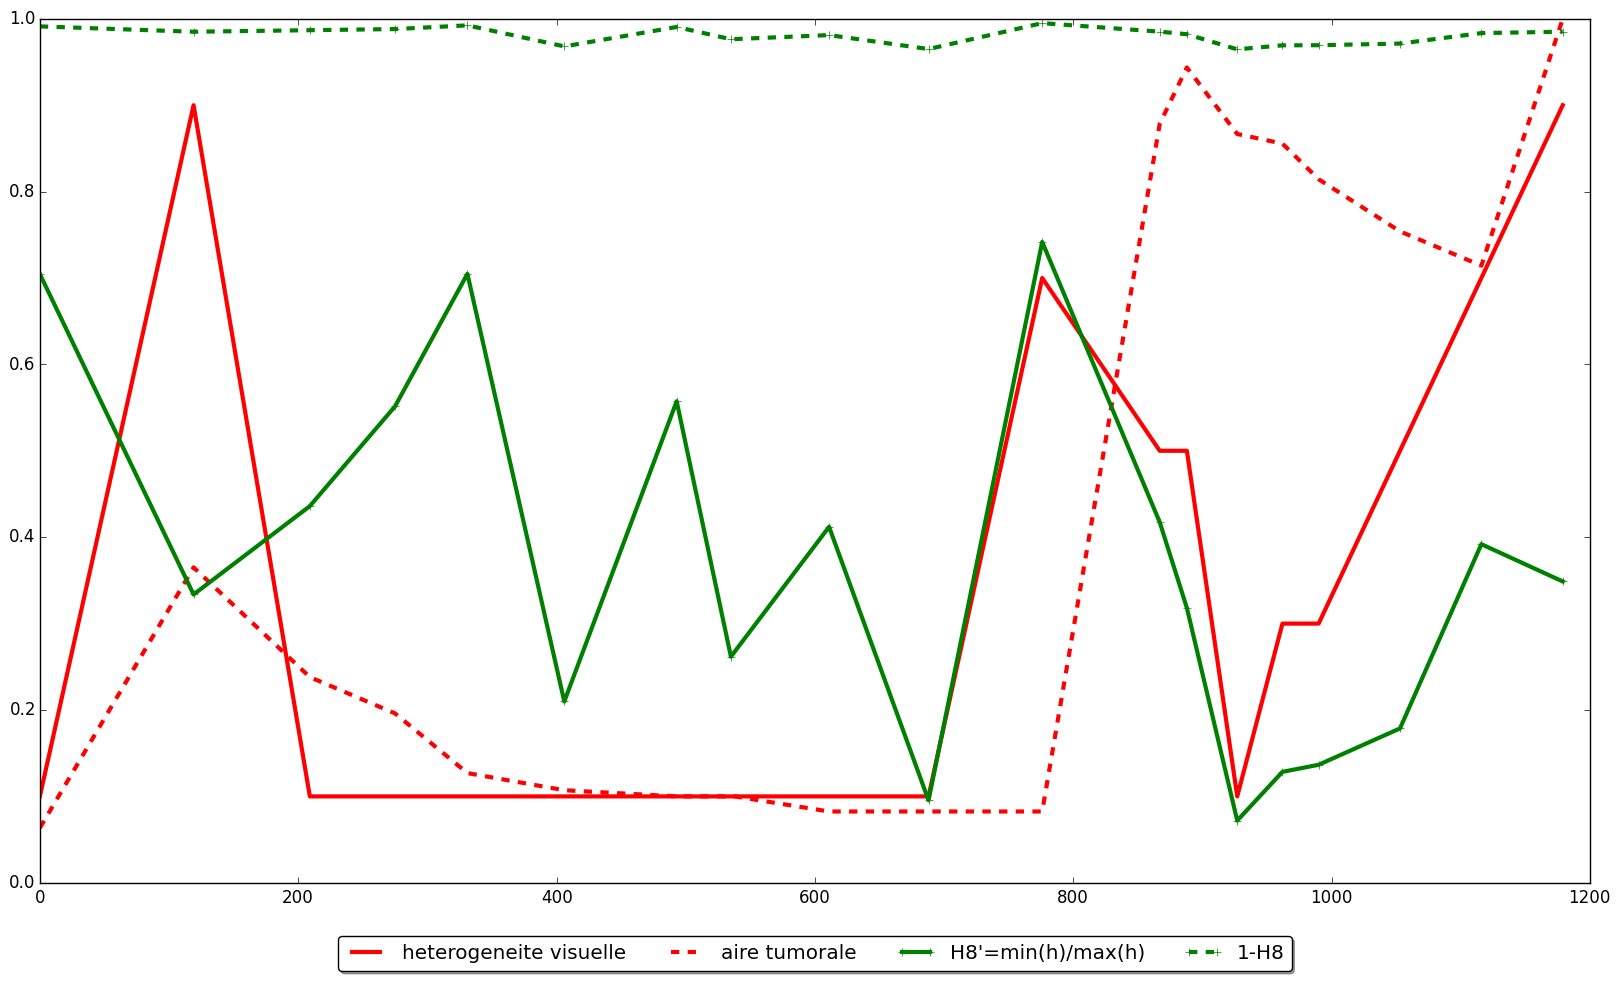
\includegraphics[width=0.48\textwidth]{graph_hetero/dcm_Nber/02-dh.png}}
\\
\centering
\subfloat[\label{fig:critere_dw}Critères basés sur $\Delta w$]{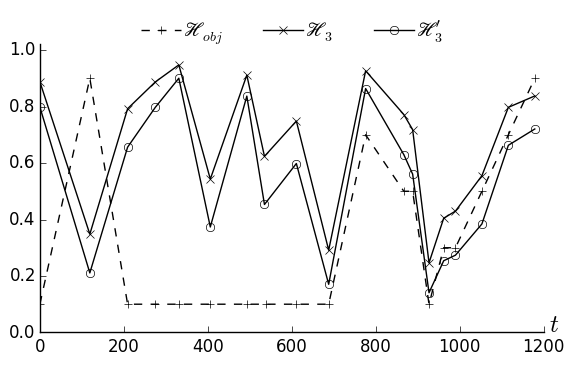
\includegraphics[width=0.48\textwidth]{graph_hetero/dcm_Nber/02_2-dw.png}}
\caption{\label{fig:premiers_criteres}Premiers critères}
\end{figure}
\begin{figure}[htpb]
\centering
%\subfloat[\label{fig:critere_dc_sur_dh}Critères basés sur la pente $\dfrac{\Delta c}{\Delta h}$]{
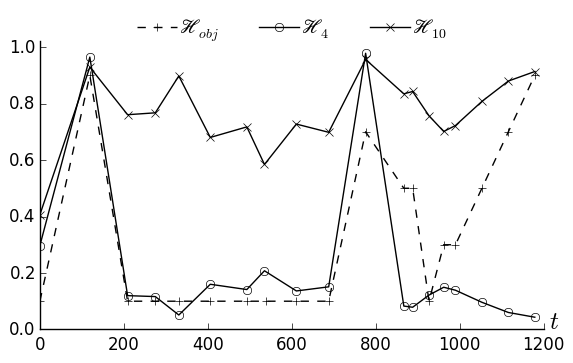
\includegraphics[width=0.70\textwidth]{graph_hetero/dcm_Nber/03-atan(dc_sur_dh).png}
%}
\caption{\label{fig:critere_dc_sur_dh}Critères basés sur la pente $\Delta c / \Delta h$}
\end{figure}

La Figure~\ref{fig:premiers_criteres} montre l'évolution de ces différentes quantités (ou de quantités qui en découle) au cours du temps. 
Les ratios $Qc, Qh$ et $Qw$ sont par définition entre 0 et 1. 
Notez que $\Delta h$ et $\Delta w$ sont nécessairement compris entre 0 et 1, puisqu'ils sont la différence de 2 élements compris entre ces même bornes. En ce qui concerne $\Delta c$ on le divisera par 256, pour également le ramener dans cet intervalle. Pour garantir l'appartenance à l'intervalle $[0,1]$, on pourra également saturer les quantités :
\begin{equation}
\label{eq:saturation_critere}
\mathscr{S}: x \longmapsto \dfrac{x}{1+x}.
\end{equation}

On remarque qu'aucune de ces quantités n'est pertinente pour décrire l'\hetero. Outre cela, on peut également remarquer les équivalences suivantes :
%\begin{equation}
%\label{eq:equiv_diff_rapport}
%\dfrac{\Delta c}{256} \simeq 1 - \dfrac{\min(c_1,c_2)}{\max(c_1,c_2)} \quad {\rm et } \quad \Delta w \simeq 1 - \dfrac{\min(w_1,w_2)}{\max(w_1,w_2)}.
%\end{equation}
\begin{equation}
\label{eq:equiv_diff_rapport}
\dfrac{\Delta c}{256} \simeq 1 - Qc \quad {\rm et } \quad \Delta w \simeq 1 - Qw.
\end{equation}
Pour $\Delta h$ et $1-Qh$, on a visiblement pas d'équivalence stricte mais les variations du ratio semble être une dilatation de celles de la différence.
On peut noter également que $Qh$ et $Qw$ sont très similaire et reproduisent assez bien la partie sur laquelle le patient est sous antiangiogénique. De plus, bien que $| \Delta c | / 256$ soit relativement bas, ses variations, si elles étaient dilatées,  pourrait s'approcher d'une description grossière de l'\hetero sur la partie avec imatinib.

Les prochains critères que nous allons étudier sont basés sur l'angle de la pente 
\todo[noline]{Il s'agit de l'inverse de la pente}
décrite entre le sommet des deux gaussiennes :
\begin{equation}
\label{eq:critere_pente}
\mathcal{H}_4 = \dfrac{1}{\pi} \left| \atan \left( \dfrac{ \Delta c }{ \Delta h }  \right) \right| + \dfrac{1}{2}
\quad {\rm et } \quad
\mathcal{H}_{10} = \dfrac{2}{\pi} \atan \left( \left| \dfrac{ \Delta c }{ \Delta h } \right| \right).
\end{equation}
\todo[noline]{l'arctangente ?}
Notons que l'arctangente, n'est ni plus ni moins qu'une autre manière de saturer une quantité. En effet, comme le montre la Figure~\ref{fig:comp_saturation}, l'arctangente est proche de la saturation $\mathscr{S}$ définie par \eqref{eq:saturation_critere}.

\begin{figure}
\centering
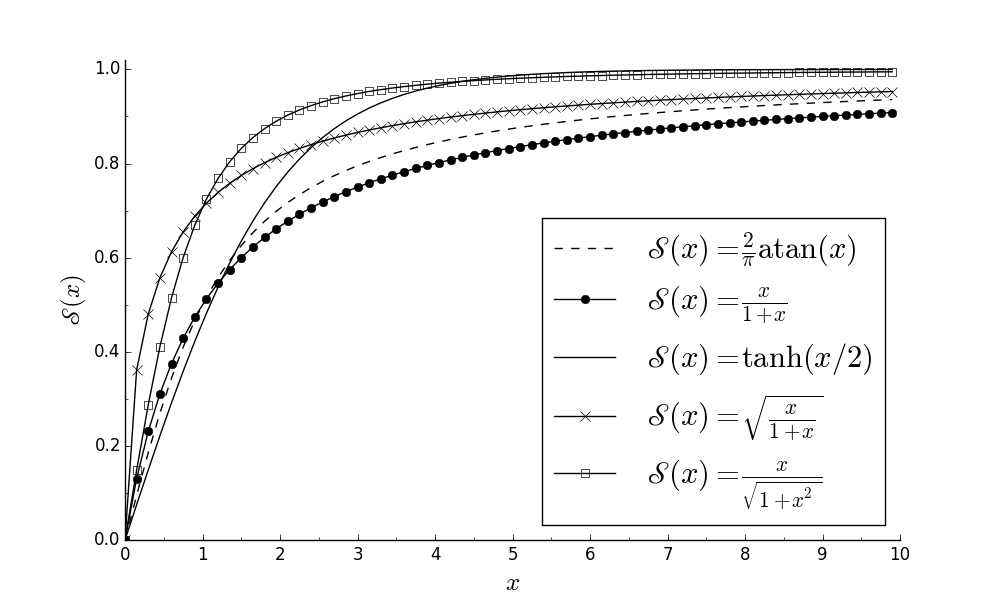
\includegraphics[width=0.75\textwidth]{comparaison_saturation.png}
\caption{\label{fig:comp_saturation}Comparaison de différentes saturations}
\end{figure}

Que la pente soit négative ou positive, à priori si les 2 composantes sont semblables, alors l'\hetero est la même. Sur la Figure~\ref{fig:critere_dc_sur_dh} est également tracé le critère qui dépend du signe de la pente, pour voir si ce signe pourrait apporter de l'information supplémentaire. Chose que nous pouvons espérer car :
\begin{itemize}
\item une pente positive va traduire qu'on a une majorité de proliférantes,
\item une pente négative va traduire qu'on a une majorité de tissu nécrosé.
\end{itemize}

Les résultats présentés sur la Figure~\ref{fig:critere_dc_sur_dh} ne sont pas encore très convaincant en ce qui concerne la description de l'\hetero... D'autres critères doivent encore être explorés.

\section{Critères basés sur la manière dont s'intersecte les gaussiennes}
Plutôt que de considérer seulement 2 points (le sommet de chaque gaussienne), élargissons notre évantail de points caractéristiques. La Figure~\ref{fig:pts_carac_intersection_gaussienne} présente l'ensemble des points utilisés dans les critères d'évaluation de l'\hetero de cette section.

\begin{figure}
\subfloat[Cas où l'une des intersection se situe entre les centres des gaussiennes.]{
\vspace{-3mm}
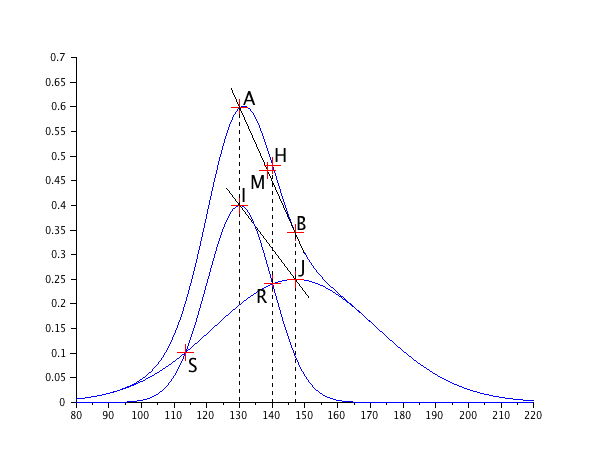
\includegraphics[width=.49\textwidth]{dessin_gauss/point_caracteristique_intersect_gauss.png}}\qquad
\subfloat[Cas où les 2 intersections sont à l'extérieure.]{
\vspace{-3mm}
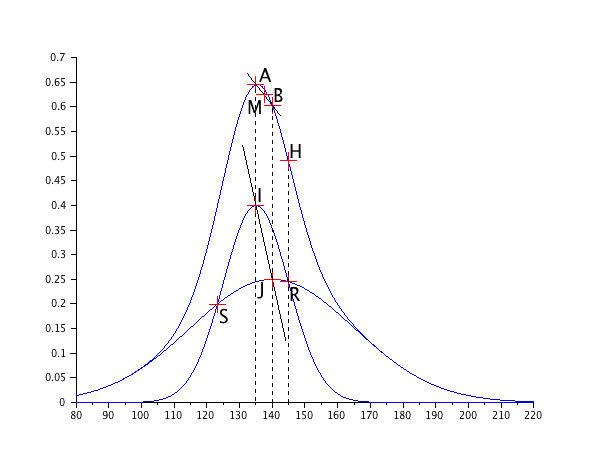
\includegraphics[width=.49\textwidth]{dessin_gauss/point_caracteristique_intersect_gauss_v2.png}}
\caption{\label{fig:pts_carac_intersection_gaussienne}Points caractéristiques de l'intersections de 2 gaussiennes.}
\end{figure}

On regardera notamment ce que peut fournir l'étude des angles $\widehat{ARB}$,  $\widehat{AHB}$, $\widehat{AGB}$ et $\widehat{MRB}$. Avant d'aller plus loin notons que la Figure~\ref{fig:pts_carac_intersection_gaussienne} présente le cas de gaussiennes dont l'abscisse de l'un des points d'intersection est situé entre les centres des deux gaussiennes ($R_x\in[c_1,c_2]$). Avant de regarder quel critère qu'il soit, étudions l'ensemble des configurations possibles entre 2 gaussiennes.

\subsection{Ensemble des configurations d'un mélange bi-gaussien.}
\begin{figure}
\subfloat[Cas avec 2 intersections, l'une se situant entre les centres des gaussiennes.]{
\vspace{-3mm}
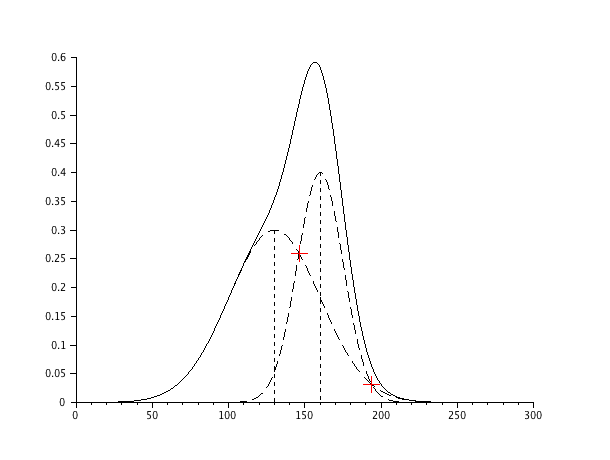
\includegraphics[width=.49\textwidth]{dessin_gauss/gmm_config1.png}}\qquad
\subfloat[Cas où les 2 intersections, toutes les deux en dehors de l'intervalle défini par le centre des gaussiennes.]{
\vspace{-3mm}
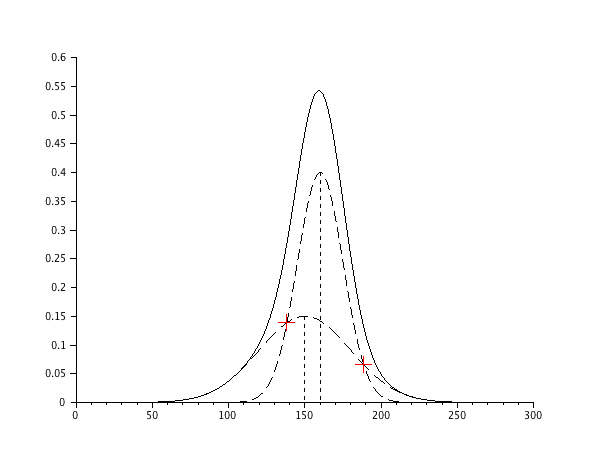
\includegraphics[width=.49\textwidth]{dessin_gauss/gmm_config2.png}}\\
\subfloat[Cas avec un seul et unique point d'intersection (ici $\sigma_1 = \sigma_2$).]{
\vspace{-3mm}
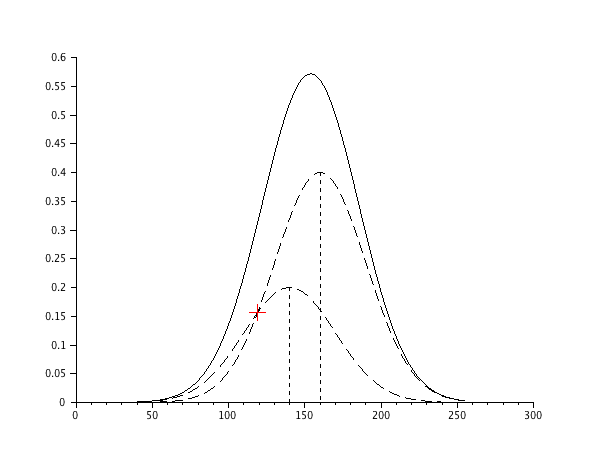
\includegraphics[width=.49\textwidth]{dessin_gauss/gmm_config3.png}}\qquad
\subfloat[Cas sans aucun point d'intersection.]{
\vspace{-3mm}
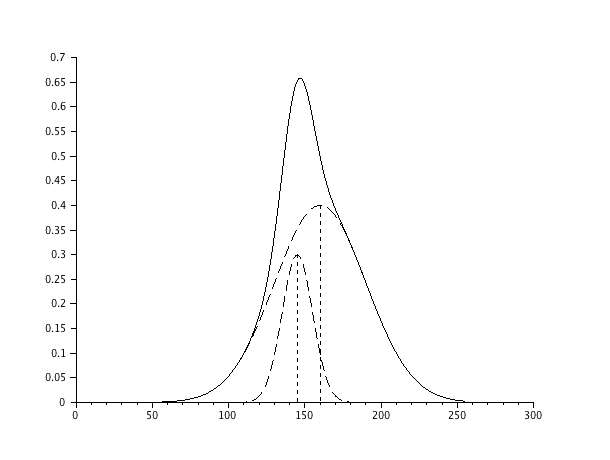
\includegraphics[width=.49\textwidth]{dessin_gauss/gmm_config4.png}}
\caption{\label{fig:config_intersection_gaussienne}Ensemble des configurations avec 2 gaussiennes.}
\end{figure}

Comme le montre la Figure~\ref{fig:config_intersection_gaussienne}, deux gaussiennes ne s'intersectent pas nécessairement. De plus, il n'est pas obligatoire d'avoir un point d'intersection dont l'abscisse est situé entre $c_1$ et $c_2$. Pour cela, résolvons l'équation suivante :
\begin{align*}
g_1(x)=g_2(x) 
& \Leftrightarrow h_1\exp \left(\frac{-1}{2} \left( \dfrac{x-c_1}{\sigma_1}\right)^2  \right) = h_2\exp \left(\frac{-1}{2} \left( \dfrac{x-c_2}{\sigma_2}\right)^2  \right), \\
& \Leftrightarrow \ln h_1 - \dfrac{1}{2}\left( \dfrac{x-c_1}{\sigma_1} \right)^2 = \ln h_2 - \dfrac{1}{2}\left( \dfrac{x-c_2}{\sigma_2} \right)^2, \\
& \overset{\sigma_i \neq 0}{\Leftrightarrow} 0 = \sigma_2^2 (x-c_1)^2 - \sigma_1^2 (x-c_2)^2 + 2\sigma_1^2\sigma_2^2 \ln( h_2 / h_1 ),
\end{align*}
qui amène à la résolution d'un polynome du second degré en $x$:
\begin{equation}
\begin{aligned}
\label{eq:g1=g2}
g_1(x)=g_2(x) \quad \Longleftrightarrow & \quad  Ax^2 + 2B'x + C =0 \\
{\rm avec :} \quad &A=\sigma_2^2 - \sigma_1^1, \\
& B'=c_2\sigma_1^2-c_1\sigma_2^2,\\
& C= c_1^2\sigma_2^2-c_2^2\sigma_1^2 +  2\sigma_1^2\sigma_2^2 \ln( h_2 / h_1 ).
\end{aligned}
\end{equation}
\paragraph{Cas particulier.}
Ecartons tout de suite le cas particulier $\sigma_1=\sigma_2$. %, que l'on notera génériquement $\sigma$. 
Dans ce cas, l'équation~\eqref{eq:g1=g2} se réécrit :
\begin{equation}
\label{eq:g1=g2_cas_part}
2\Delta c \; x + c_1^2-c_2^2 +  2 \sigma^2 \ln \big( (1-w) / w \big) = 0
\end{equation}
\begin{itemize}
\item Si de plus $\Delta c=0$, alors \eqref{eq:g1=g2_cas_part} implique que $h_1=h_2$, et donc les deux gaussiennes sont absolument identiques et superposées.
\item Si $\Delta c\neq0$, alors on a un seul et unique point de croisement, dont l'abscisse est :
\begin{equation}
\label{eq:pt_croisement_unique}
x=\dfrac{c_1+c_2}{2}-\dfrac{\sigma^2}{\Delta c}\ln \left( \dfrac{1-w}{w} \right).
\end{equation}
\end{itemize}
\paragraph{Cas général.} Il convient ici de calculer le discriminant réduit:
\begin{equation}
\label{eq:discr_reduit}
\Delta' := B'^2 - AC = \sigma_1^2 \sigma_2^2 \left[ (\Delta c)^2 - 2(\sigma_2^2-\sigma_1^2) \ln (h_2/h_1)  \right].
\end{equation}
Ce discriminant n'est pas nécessairement positif ! Donc il existe des cas où les gaussiennes ne s'intersectent pas.
\todo[inline]{analyse du signe du discriminant à compléter}

\subsection{Etudes de différents critères}
\begin{itemize}
\item Basé sur intégrale commune
\item Basé sur des angles
\item Basé sur des positions relatives de point ...
\end{itemize}
\todo[inline]{A completer}

\section{Critère retenu}
\begin{figure}
\centering
\subfloat[\label{fig:pente_gaussienne_identique_a} Cas clairement \heterogene ]{
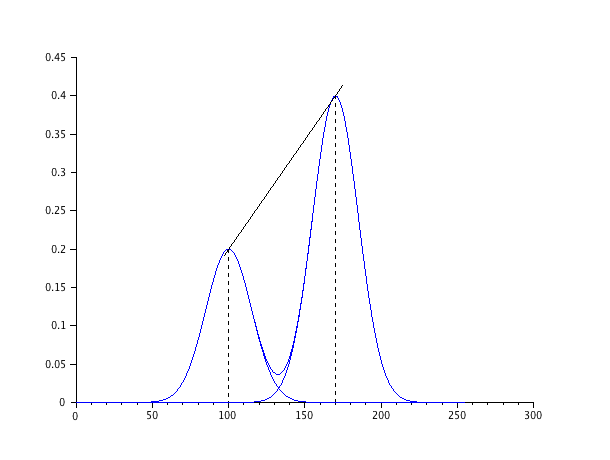
\includegraphics[width=.49\textwidth]{dessin_gauss/gmm_pente1a.png}
}
\subfloat[\label{fig:pente_gaussienne_identique_b} Cas plutôt homogène]{
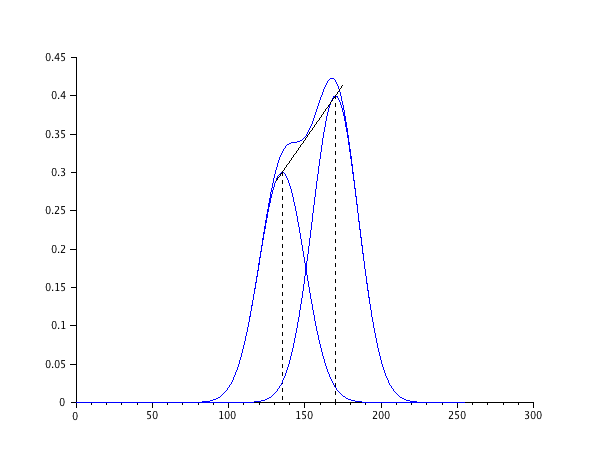
\includegraphics[width=.49\textwidth]{dessin_gauss/gmm_pente1b.png}
}
\caption{\label{fig:pente_gaussienne_identique}Deux configurations très différentes mais fournissant la même pente entre les gaussiennes.}
\end{figure}
L'idée de ce dernier critère m'est venu de la constation suivante.
En repartant du critère de la pente décrite entre le sommet des gaussiennes, sur la Figure~\ref{fig:pente_gaussienne_identique} est présenté deux configurations très différentes, mais présentant la même pente. Pourtant la Figure~\ref{fig:pente_gaussienne_identique_a} est très clairement représentative d'une image \heterogene alors que la Figure~\ref{fig:pente_gaussienne_identique_a} serait plutôt représentative de qqch d'homogène puisque l'approximation par une seule et unique gaussienne ne serait pas des plus mauvaise. 
Comment différencier ces deux cas ? Cet exemple mis en exergue nous invite à dire que $\Delta c$ doit avoir plus de poids que $\Delta h$ dans le calcul du critère de l'\hetero. Ainsi, j'ai décidé de regarder le critère suivant :
\begin{equation}
\label{eq:criteres_finaux}
\mathcal{H}_{11} = \mathscr{S}\left( \left| \dfrac{(\Delta c /256)^2}{\Delta w} \right| \right)
\quad {\rm et } \quad
\mathcal{H}_{2} = \mathscr{S} \left( \left| \dfrac{(\Delta c /256)^2}{\Delta h} \right| \right)
\end{equation}
\begin{figure}
\centering
\subfloat[\label{fig:critere_dc2_sur_dh} Critères basés sur $(\Delta c)^2 / \Delta h$ ]{
\includegraphics[width=0.48\textwidth]{graph_hetero/dcm_Nber/06-dc2_sur_dh.png}
}
\subfloat[\label{fig:critere_dc2_sur_dh} Critères basés sur $(\Delta c)^2 / \Delta w$ ]{
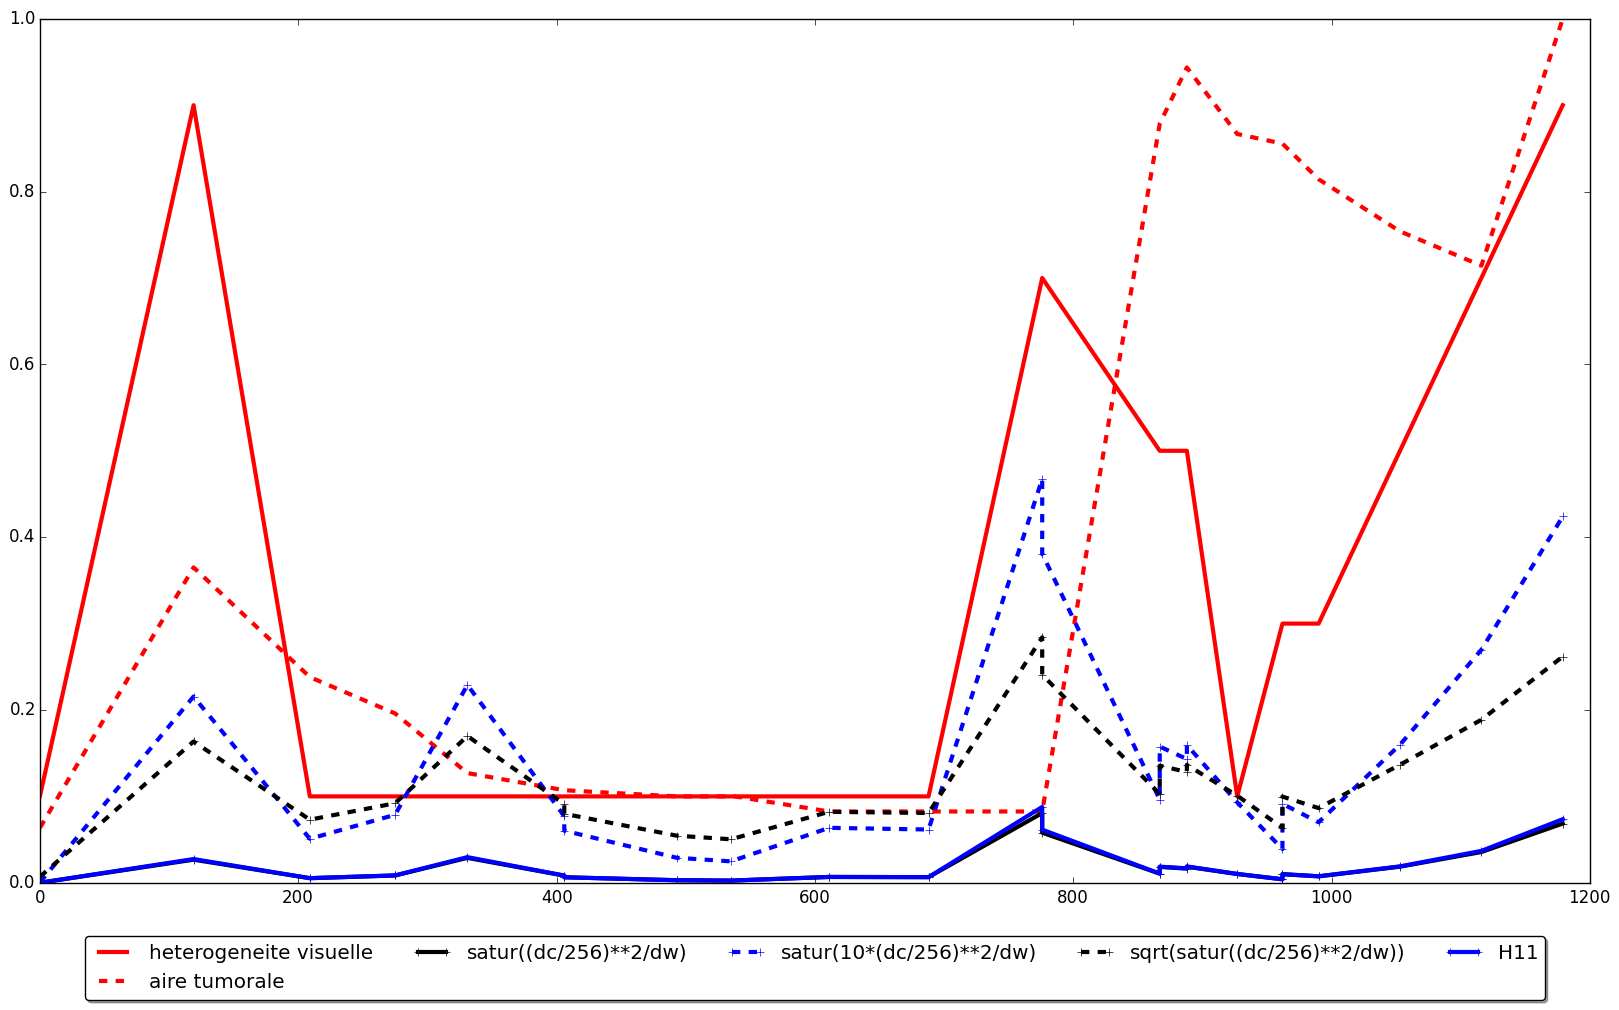
\includegraphics[width=0.48\textwidth]{graph_hetero/dcm_Nber/07-dc2_sur_dw.png}
}
\caption{\label{fig:critere_avec_dc2}Critères dans lesquels $\Delta c$ joue un rôle prépondérant.}
\end{figure}


\begin{figure}
\centering
\includegraphics[width=0.75\textwidth]{graph_hetero/dcm_Chen/06-dc2_sur_dh.png}
\caption{\label{fig:critere_dc2_sur_dh_Chen} Critères basés sur $(\Delta c)^2 / \Delta h$ sur \Chen }
\end{figure}

\section{L'\hetero sur les simulations numériques}
\todo[noline]{Nouveau chapitre ?}
\todo[noline]{Titre sous-section ?}
\subsection{Titre ....}
Maintenant que nous avons un critère qui décrit correctement l'\hetero clinique (d'une métastase à partir de l'imagerie médicale), faisons parler ce critère sur nos simulations numériques. En ce qui concerne cet aspect, les images  résultantes (gouvernées par EQREF \todo[noline]{eqref} ) des simulations numériques dépendent de 3 paramètres : $\tau_N, \tau_P$ et $\tau_S$ qui représentent les niveaux de gris associés à chacune de nos populations de notre modèle EDP. Ainsi, pour une simulation numérique donnée, il n'y a pas unicité de l'image produite en niveau de gris, et donc non unicité de l'histogramme. Tout dépend de ces 3 paramètres. Dans un premier temps,  on examinera ce que cela donne avec les valeurs heuristiques considérées  dans la première partie de ce manuscrit : $\tau_N=38, \tau_P=166$ et $\tau_S=204$.
\todo[noline]{Et l'optim du niveau de gris faite entre temps ?}
Dans un second temps, on pourra faire varier ces paramètres pour examiner l'influence de ceux-ci sur l'\hetero numérique.
On ne montrera ici que l'\hetero numérique de \Nber. Celle de \Chen n'a absolument aucune chance d'être correctement reproduite pour la simple et bonne raison que le premier scan est très \heterogene, alors que notre condition initial dans le modèle numérique est complètement homogène. Il faudrait prendre une condition initiale plus en relation avec l'image médicale, à minima une condition initiale qui présenterait le même niveaux d'\hetero pour pouvoir poursuivre l'étude avec ce patient.

\begin{figure}
\centering
\includegraphics[width=0.75\textwidth]
{graph_hetero/simu_Nber_N38_P166_S204/06-dc2_sur_dh.png}
\caption{\label{fig:hetero_nber_simu}\Hetero numérique pour \Nber\ -- $\tau_N=33, \tau_P=166$ et $\tau_S=215$. L'\hetero clinique est rappelée, à titre de comparaison, ici en rouge.}
\end{figure}

Sur la Figure~\ref{fig:hetero_nber_simu} est présenté l'\hetero numérique de \Nber.
La fonction objectif pour l'\hetero clinique ainsi que l'évolution de l'aire tumorale sont ici rappelées sur ce graphique à titre comparatif. La phase avec imatinib est  correctement décrite :
\begin{itemize}
\item Présence d'un pic d'\hetero jour~119.
\item Décroissance de l'\hetero lorsque l'imatinib agit de manière efficace.
\item Saut important de l'\hetero qui grandit juste avant la recroissance de l'aire tumorale.
\end{itemize}
En ce qui concerne la partie avec sunitinib, au début de l'administration du traitement l'\hetero décroit. Cependant :
\begin{itemize}
\item La recroissance de l'\hetero numérique a lieu un peu tôt par rapport à celle constatée cliniquement.
\item Sur la partie finale (lors de la rechute au sunitinib, après le jour~1116), l'\hetero numérique décroit alors que celle clinique continue d'augmenter. 
\end{itemize}
En ce qui concerne le deuxième point, cela peut venir soit de la manière dont on calcule l'\hetero, soit du modèle EDP lui même qui ne retranscrirait pas bien l'évolution de l'\hetero. La Figure~\ref{fig:baisse_hetero_fin_simu} tends à dire que c'est plutôt le modèle EDP puisque le jour~1120 est beaucoup plus \hetero que le 
jour~1227. En effet, le contraste entre les deux masses dominantes (pourtour et intérieur de la tumeur) 
est beaucoup plus important jour~1120 que jour~1227. De plus le rapport du volume de ces dominantes est beaucoup plus proche de 1 au jour~1120 qu'au jour~1227 (si le ratio est égal à 1 alors les masses sont de volume égal). Ces impressions visuelles sont confirmées par les histogrammes également présentés sur la Figure~\ref{fig:baisse_hetero_fin_simu}. 
Tout ceci renforce donc l'idée que l'image du jour~1120 est plus \hetero que celle du jour~1227.

\begin{figure}
\centering
\subfloat[Jour~1120]
{\begin{tabular}{c}

\includegraphics[width=0.31\textwidth]
{simu/N38_P166_S204/fit_henbert_form3_seuil0.1/tumor086.png}\\
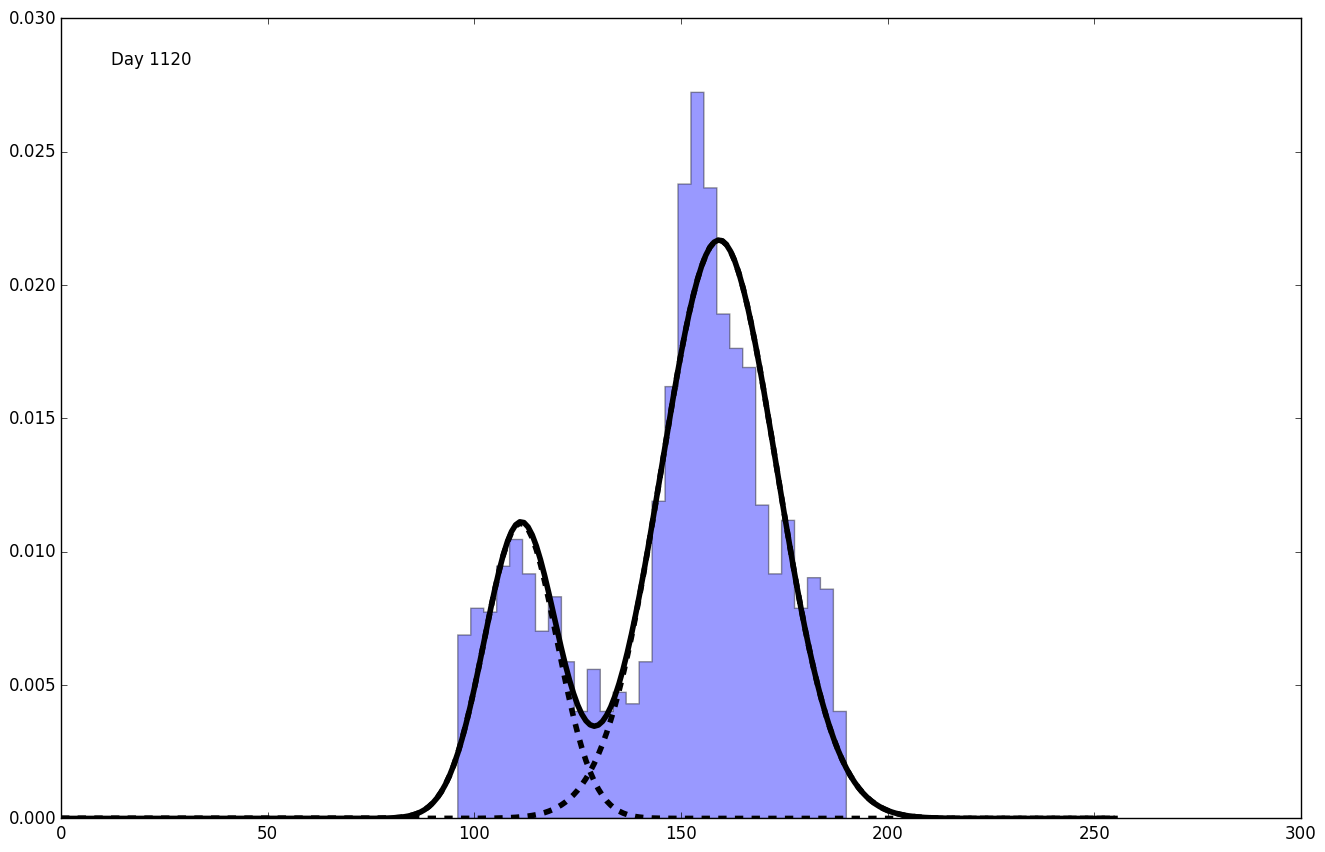
\includegraphics[width=0.31\textwidth]
{simu/N38_P166_S204/fit_henbert_form3_seuil0.1/histo/Nber_day1120(85).png}
\end{tabular}}
\subfloat[Jour~1186]
{\begin{tabular}{c}
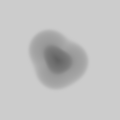
\includegraphics[width=0.31\textwidth]
{simu/N38_P166_S204/fit_henbert_form3_seuil0.1/tumor091.png}\\
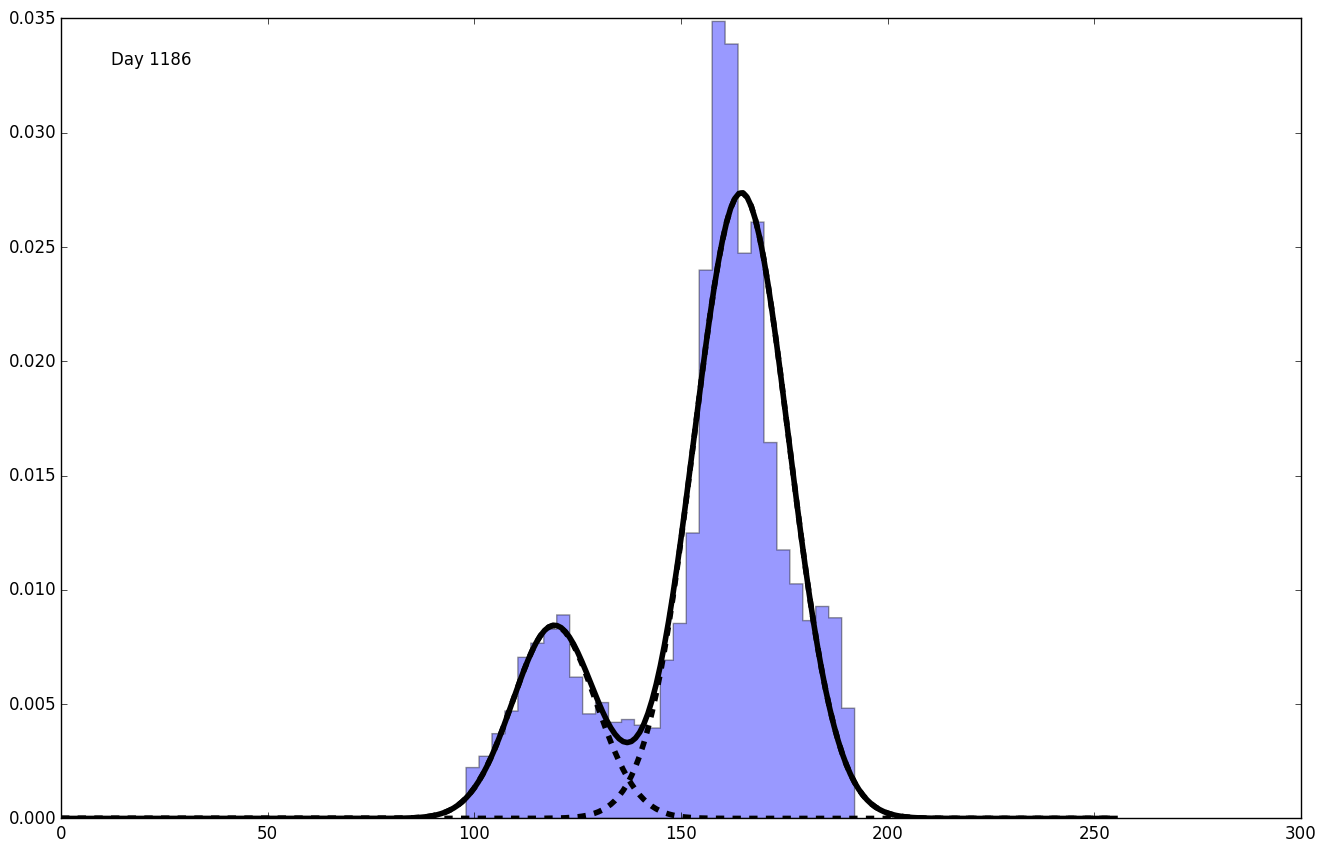
\includegraphics[width=0.31\textwidth]
{simu/N38_P166_S204/fit_henbert_form3_seuil0.1/histo/Nber_day1186(90).png}
\end{tabular}}
\subfloat[Jour~1227]
{\begin{tabular}{c}

\includegraphics[width=0.31\textwidth]
{simu/N38_P166_S204/fit_henbert_form3_seuil0.1/tumor095.png}\\
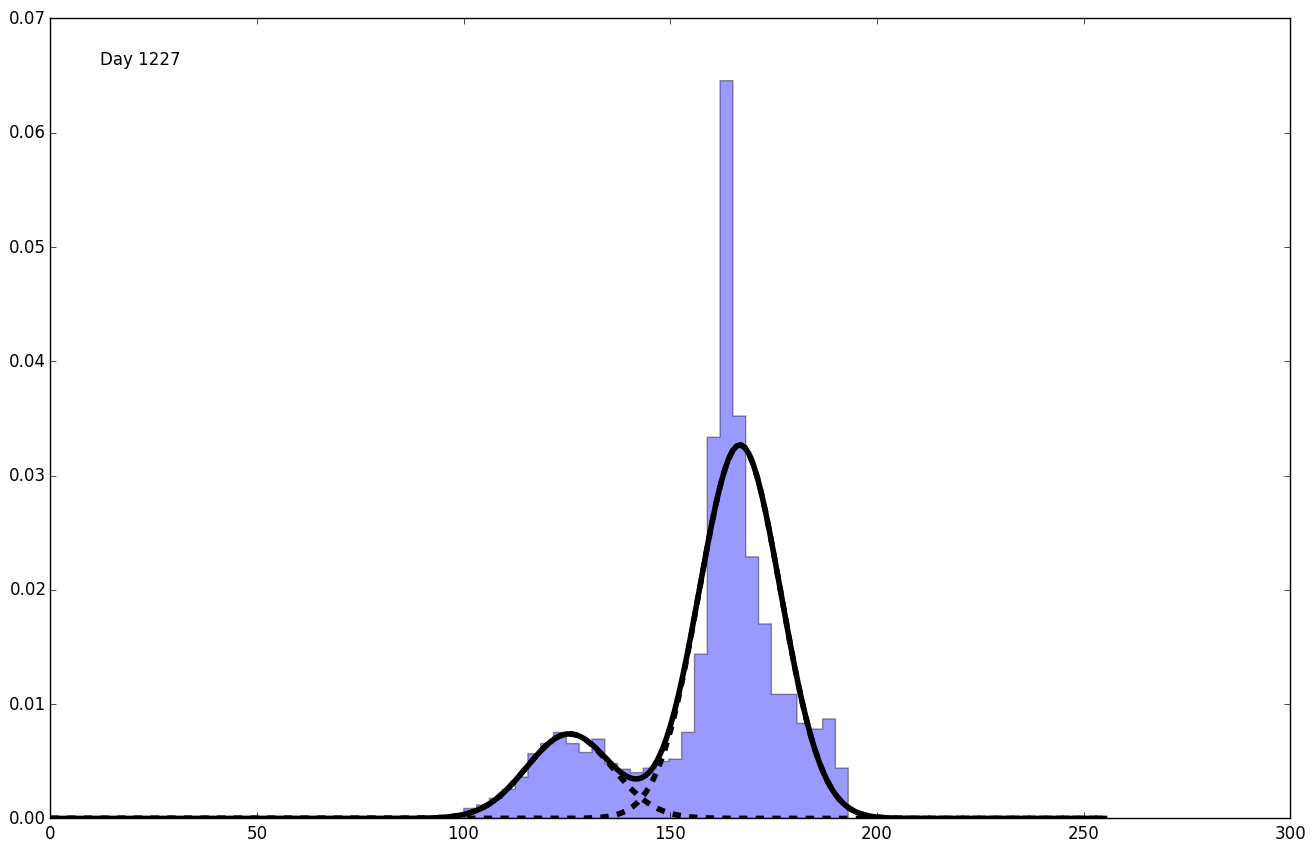
\includegraphics[width=0.31\textwidth]
{simu/N38_P166_S204/fit_henbert_form3_seuil0.1/histo/Nber_day1227(94).png}
\end{tabular}}
\caption{\label{fig:baisse_hetero_fin_simu} \Hetero numérique de \Nber. }
\end{figure}


\subsection{Influence des niveaux de gris sur l'\hetero numérique}
La principale conséquence du changement des niveaux de gris $\tau_N$, $\tau_P$ et $\tau_S$ est la dilatation de l'histogramme des niveaux de gris. Les variations de l'\hetero ne sont donc que peu dépendante de ces paramètres, comme le montre 
la Figure~\ref{fig:impact_grey_lvl_on_hetero}, sur laquelle toute les courbes sont comparables. Comme différence, on pourra relever tout de même que plus $\tau_N$ est écarté de $\tau_P$, plus les variations de l'\hetero numérique sont importantes. Ceci est notamment visible lors de la rechute à l'imatinib, entre les jour~776 et 888 où le pic descendant de l'\hetero numérique est plus prononcé si $\tau_P-\tau_N$ est grand. Ceci est conforme à ce que l'on pouvait attendre, puisque cette différence va impacter directement la position des gaussiennes sur l'histogramme, position relative en grande partie donnée par $\Delta c$ qui intervient dans le calcul de notre critère de l'\hetero numérique.

\begin{figure}
\centering
\subfloat[$\tau_N=23, \tau_P=142$ et $\tau_S=215$]
{\includegraphics[width=0.48\textwidth]
{graph_hetero/simu_Nber_N23_P142_S215/06-dc2_sur_dh.png}}
\subfloat[$\tau_N=30, \tau_P=122$ et $\tau_S=215$]
{\includegraphics[width=0.48\textwidth]
{graph_hetero/simu_Nber_N30_P122_S215/06-dc2_sur_dh.png}}\\
\subfloat[$\tau_N=26, \tau_P=127$ et $\tau_S=215$]
{\includegraphics[width=0.48\textwidth]
{graph_hetero/simu_Nber_N26_P127_S215/06-dc2_sur_dh.png}}
\subfloat[$\tau_N=36, \tau_P=142$ et $\tau_S=215$]
{\includegraphics[width=0.48\textwidth]
{graph_hetero/simu_Nber_N36_P142_S215/06-dc2_sur_dh.png}}
\caption{\label{fig:impact_grey_lvl_on_hetero} Influence du choix des niveaux de gris $\tau_N, \tau_P$ et $\tau_S$ sur l'\hetero numérique.}
\end{figure}

\end{document}